\documentclass[a4paper,12pt]{article}

\usepackage{url}
\usepackage{epsfig}
\usepackage{graphics}
\usepackage{fancyhdr}
\usepackage{amsmath}
\usepackage{array,xcolor,colortbl}
\usepackage{multirow}
\usepackage{multicol}
\usepackage{float}
\usepackage{adjustbox}
\usepackage{enumitem}
\usepackage{caption}
\usepackage{subcaption}
\usepackage{tablefootnote}
\usepackage[linguistics]{forest}



\graphicspath{{pictures/}}

\title{Report Assignment 2 DD2380}
\author{\hspace*{-0.5cm}
GROUP 4:3\\
\begin{tabular}{cccc}
Vilmer Jonsson & Tor Strimbold\\
2001-06-26 & 1999-10-06 \\ 
vilmerj@kth.se & torstri@kth.se \\
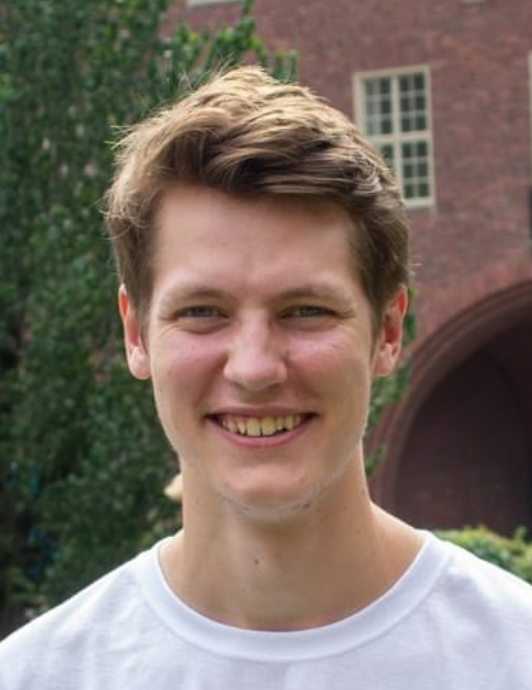
\includegraphics[width=0.13\linewidth]{Vilmer_Jonsson.jpg}
& 
\includegraphics[width=0.13\linewidth]{tor.jpg}
\end{tabular}} 
% Normally there will not be any pictures but we want
% these so that we can connect faces to names in the course
% We also want birthdates so that we can tell people with the same
% name apart
\date{\today}

\pagestyle{fancy}
\setlength{\headheight}{15pt}
\fancyhf{}
\lhead{DD2438} % DO NOT REMOVE!!!!
\rhead{V. Jonsson, T. Strimbold} %% UPDATE WITH YOUR NAMES
\fancyfoot[C, CO]{\thepage}

\begin{document}

\maketitle
\thispagestyle{fancy}

\begin{abstract}



\end{abstract}


\clearpage

%%%%%%%%%%%%%%%%%%%%%%%%%%%%%%%%%%%%%%%%%%%%%%%%%%%%%%%%%%%%%
%%%%%%%%%%%%%%%%%%%%%%%%%%%%%%%%%%%%%%%%%%%%%%%%%%%%%%%%%%%%%
\section{Introduction}
\label{sec:intro}

The game Snake was first released in 1976 where two players controlled a "snake" which continually grows for every turn, to grow as large as possible before being eliminated by either colliding with the surrounding wall. This project is based on the retro game through the coding challenge provided by Battlesnake.com. Several formats are more or less similar to the original game, but the main difference is that snakes now have a \textit{health} property which starts at 100 points and decrements for every in-game turn. When a snake consumes any of the food on the board, the snake grows by one square and their health is restored. This extension is a part of every \textit{battle snake} theme but some of the most popular formats are \textit{standard}, where four snakes battle each other, \textit{duels}, where two snakes face-off, which the similar format to that of the original game, and \textit{royale} where four snakes fight on a board where a "hazardous" zone grows from the edges towards the center, inflicting further reductions to the snakes' health when they pass through the zone.


Thus, the problem underlying the problem is to design an agent that can effectively handle different situations and make decisions regarding short-term versus long-term rewards. It is, for example, not always the best move to eat food to grow or risk an attack against an enemy if it could result in a precarious situation if the attack fails. Furthermore, in this project, teams were tasked with writing code to guide the snake in a 2v2 format which introduces additional parameters to the problem. Through this extension, the snakes' survival chances are increased if they can collaborate to eliminate the opposing team.


\subsection{Game \& Competition Rules}
At the end of the project, a competition was held to determine which of the submitted solutions was the strongest. The matches were run on the standard format which can be summarized as follows:

\begin{enumerate}
    \item The map consists of an 11 by 11 grid.
    \item Two teams compete with two snakes per team.
    \item Each snake has a “health” value that starts at 100 but decrements for every in-game turn. If a snake’s health is reduced to zero, the snake is eliminated.
    \item Every round of food can be spawned on the map, if a snake eats any of the food its length is increased by one and its health is restored to 100.
    \item If a snake runs out of bounds or into another snake's body, excluding the head, the snake is eliminated.
    \item If two snakes collide head-on, the shortest snake is eliminated. In the case where both snakes are of equal length, both snakes are eliminated.
    \item A team wins a match if both of the enemy snakes are eliminated before the own snakes. In the case where both teams’ snakes are eliminated simultaneously, the game results in a draw.
\end{enumerate}
Lastly, the competition consisted of two parts, first a round where every team faced off against every other team, and a play-off consisting of the top 8 teams from the previous round.


\subsection{Contribution}
The work presented in this report is an implementation of a collaborative AI agent that utilizes the Monte Carlo Tree Search (MCTS) algorithm. The algorithm was implemented in Node with JavaScript and was hosted on a server owned by Replit. The presented work aims to further explore the capabilities of the MCTS algorithm and contribute to the field of artificial intelligence. Many modern video-games rely on having non-playable characters (NPC) which human players can interact with. These agents need to be able to navigate through and interact with their environment to engage with the player. The algorithms used can however also be employed when running other type of simulations not related to video games. Lastly, the results presented in the report are not only relevant to the techniques implemented in the solution, but also compared to the work performed in conjunction with our own. In total 25 teams were tasked with solving the presented problems which resulted in a plethora of different approaches and algorithms at play. 



\subsection{Outline}
The outline of the rest of the report is as follows: section 2 presents the related works concerning our implementation of the problem, the following section 3 gives the reader an overview of our solution and the underlying algorithms, section 4 presents the results of the competition hosted at the end of to protect as well as some online tournaments, our work is lastly discussed and summarized in section 5 and 6 respectively.


%%%%%%%%%%%%%%%%%%%%%%%%%%%%%%%%%%%%%%%%%%%%%%%%%%%%%%%%%%%%
%%%%%%%%%%%%%%%%%%%%%%%%%%%%%%%%%%%%%%%%%%%%%%%%%%%%%%%%%%%%%
\newpage
\section{Related work}
\label{sec:relwork}
% \emph{Related Work section describing and referring to at least 5 research papers}

Example citation \cite{RussellNorvigAIBook3rd}.


%%%%%%%%%%%%%%%%%%%%%%%%%%%%%%%%%%%%%%%%%%%%%%%%%%%%%%%%%%%%%
%%%%%%%%%%%%%%%%%%%%%%%%%%%%%%%%%%%%%%%%%%%%%%%%%%%%%%%%%%%%%
\newpage
\section{Proposed method}
\label{sec:method}

The AI is implemented using the Monte Carlo Tree Search (MCTS) algorithm. The algorithm is divided into four main steps: selection, expansion, simulation, and backpropagation. Every turn, the algorithm is called and starts to run iteratively for a certain amount of time. 

Every node in the tree represents a state in the game. The root node is the current state of the game, and the children of the root node are the possible moves that can be made from the current state. A move is defined as all snakes in a team moving one step in a certain direction. If a move results in a collision, the move is invalid, and the node is not expanded. Thus, the number of children a node can vary, but is at most nine, since each snake can turn left or right, or go straight, and there are at most two snakes in a team. %% Detta är lite wonky

%% Vi kanske borde ha en figur här som visar hur trädet ser ut

\subsection{Selection}
In every iteration, there is a selection phase where the algorithm selects the best child node to explore. The selection starts from the root and then traverses down the tree, picking the best child at each level, until it reaches a leaf node, a node with no children.


The best child is selected based on the Upper Confidence Bound (UCB) formula. The formula is defined as:

\begin{equation} \label{eq:ucb}
    UCB = \text{score}_i + C \sqrt{\frac{\ln{N}}{n_i}}
\end{equation}

Where $\text{score}_i$ is the average score of the node, $N$ is the total times the parent node has been visited, $n_i$ is the number of times the node has been visited, and $C$ is a constant that controls the exploration-exploitation trade-off. The constant $C$ was set to $\sqrt{2}$ in this implementation, but no empirical testing was done to determine the optimal value. If the node has not been visited, the UCB value is set to infinity to ensure that the node is selected at least once if its parent node has been visited.


\subsection{Expansion}

%% Blir kanske lite repetativt från början på Proposed method
The expansion phase is where the algorithm creates new child nodes for a leaf node. To create the child nodes, every possible move from the current state is generated. Generating a state is done by copying the current state and applying a move of one of the team's snakes. If the snake has no valid moves, it will be removed in the new state. 



\subsection{Simulation and Evaluation}

When new children have been added to the leaf node, the best child according to equation \ref{eq:ucb} is selected. To determine the score of the node, the algorithm simulates the game from the selected child node for 12 or 12.5 rounds, depending on whether the friendly or enemy team makes the first move. The purpose of this is to ensure both teams have done the same number of moves when the simulation ends. The simulation is done by selecting a random \textit{valid} move for each snake in the team. A move is considered valid if it does not result in a collision with a wall or another snake. This is done to make the simulation more realistic while still covering many possible states. There were considerations of for example simulating the snakes targeting food, but this was not implemented due to not wanting to bias the simulation and risk limiting the exploration of alternative, potentially better, moves.


The score of the simulation is based on a heuristic function that evaluates the state of the game in the end of the simulation. The heuristic function is described in equation \ref{eq:heuristic}.


\begin{multline} \label{eq:heuristic}
    \text{score} = \text{accLengthFriendly} - \text{accLengthEnemy}\\ + 10 (\text{accHealthFriendly} - \text{accHealthEnemy})
\end{multline}

Where both the values of length and health is accumulated, which means that it is the total length or health of all snakes in a team. The heuristic function is simple and is designed to decide which of the teams have the most beneficial position at the end of the simulation. Accumulated values are used to give a higher score to the team with the most snakes alive. There were other heuristic functions tested, but when played against each other, the heuristic function described in equation \ref{eq:heuristic} performed the best.

An important attribute of the scoring heuristic is that it is symmetric. This means that the same can be used for both the friendly and enemy teams. When back-propagating the score, the score is negated when back-propagating to the parent node, to ensure that the parent node gets the score of the enemy team. This is done to ensure that the simulation tries to maximize the score of the enemy team, which is the same as minimizing the score of the friendly team.


%% Kanske nåt sånt här, men platsar typ inte här utan experimental results
%% The heuristic function may be the area were the most improvement could be done to the algorithm. The heuristic function is simple and the snakes are great when they are longer than their opponents and have momentum. However, the snakes seem to sometime not prioritize food in the beginning of the game and instead just try to survive. 




\subsection{Edge Cases}

The algorithm uses some edge cases to handle certain situations that may occur during the game. These edge cases often occur because the modeling of the game state is suboptimal. The most apparent flaw is that in the game the snakes do their moves simultaneously, but in the simulation, the snakes move one after another. This can lead to situations where a snake can move into a position that would result in a collision with another snake that has not done its move in the specific turn yet.


\subsubsection{Head-To-Head Collisions} %% Ta bort \subsubsection om vi inte har fler edge-cases

In the early stages of testing the algorithm, it was discovered that the snakes would often collide head-to-head and this would thus heavily impact the outcome of the game since the shorter snake would die. % Wonky sentence
The reason why head-to-head collisions are difficult to model is that the snakes move simultaneously in the game, but in the simulation, the snakes move one after another. This can lead to a situation where one snake moves into a position that another snake also can move to, resulting in a head-to-head collision. To handle this, the algorithm is very safe regarding the friendly snakes. The friendly snakes will never move into a position that would risk a head-to-head collision with a longer snake. However, the algorithm assumes that enemy snakes can take such risks, this leads the algorithm to be more aggressive and try to set up for a head-to-head collision when the enemy snake is shorter.






%%%%%%%%%%%%%%%%%%%%%%%%%%%%%%%%%%%%%%%%%%%%%%%%%%%%%%%%%%%%%
%%%%%%%%%%%%%%%%%%%%%%%%%%%%%%%%%%%%%%%%%%%%%%%%%%%%%%%%%%%%%
\newpage
\section{Experimental results}
\label{sec:exps}

This section presents the experimental results collected at the end of the project through the competition mentioned in section 1.3.


\subsection{Competition Results}
The largest testing of our solution was through the competition hosted on the 19th and 20th of May containing 26 other teams from the course. The competition consisted of two different parts, first a round where every team played a match against every other team, and secondly a play-off between the top 8 teams. During the first part, each team were responsible for hosting twelve games each, thus we hosted games against twelve other teams and the remaining teams hosted games against us. In this manner, every team was paired against each other in the first round. Furthermore, a win was awarded 3 points, a draw 1 point and a loss did not net any points. Consequently, the eight best teams from this round then played a knockout tournament, where matches consisted of a best-of-three format and the loser was eliminated while the winner progressed to the next round. 

Table \ref{tab:round1} presents our results from the first round, where our solution performed well beating 19 of the teams while losing the remaining 5 matches. This resulted in a total of 57 points and a shared first place with five other teams, see Table 2 for reference, and in turn a place in the ensuing knockout stage. The results from the play-offs can be viewed in Figure 1, where we are group 3.

\begin{table}[ht!]
    \centering
    \begin{tabular}{|l|l|l|l|l|}
        \hline
        & Wins        & Draws      & Losses     & Points      \\ \hline
        Home           & 10          & 0          & 2          & 30          \\ \hline
        Away           & 9           & 0          & 3          & 27          \\ \hline
        \textbf{Total} & \textbf{19} & \textbf{0} & \textbf{5} & \textbf{57} \\ \hline
    \end{tabular}
    \caption{Results from the first round of the competition.}
    \label{tab:round1}
\end{table}


\begin{center}
    \begin{forest}
      for tree={
        grow=west,
        parent anchor=west,
        child anchor=east,
        edge={draw, -},
        l sep+=10pt,
        s sep+=10pt,
        anchor=west,
        calign=center,
        calign primary angle=30,
        calign secondary angle=60,
        edge path={
          \noexpand\path [draw, -] (!u.parent anchor) -- ++(5pt,0) |- (.child anchor)\forestoption{edge label};
        },
      }
      [Group 23
        [Group 2
          [Group 2
            [Group 2]
            [Group 4]
          ]
          [Group 3
            [Group 3]
            [Group 9]
          ]
        ]
        [Group 23
          [Group 12
            [Group 12]
            [Group 13]
          ]
          [Group 23
            [Group 23]
            [Group 24]
          ]
        ]
      ]
    \end{forest}
\end{center}


  

Our solution differed from most of the top 8 teams where only two other groups employed a tree search algorithm. The first was group 13 which utilized a paranoid Minimax algorithm where each snake saw all the other snakes as opponents, hence the paranoid part, and group 9 who used a game tree of depth 2 to determine which move to make. The remaining teams’ approaches were similar to a “rule-based” method where a modified A* algorithm would guide the snake based on different weights and heuristics. One common idea was to use the flood fill algorithm to find dead-ends and reachable grid cells from any position. This can then be used to determine which grid cell a snake should navigate towards and the path to the destination would be determined using A* where different weights, such as proximity to enemy snakes, guide the search.


Lastly, out of curiosity, we enrolled our solution in some daily competitions hosted by \url{https://play.battlesnake.com/} where anyone can submit their solution. The snakes then battle in the free-for-all settings listed below.

\begin{enumerate}
    \item \textbf{Standard:} four snakes face off on an 11 by 11 grid and the last remaining snake is the victor. The rules regarding elimination are the same as those described in section 1.1.
    \item \textbf{Duels:} The same format as standard, only in duels there are only two snakes.

    \item \textbf{Royale:} The same format as standard, with the exception of a “hazardous” zone which grows from the borders of the map towards the centre. If a snake moves through this zone an additional health point is lost during the turn.

\end{enumerate}
For an extensive description of the different game modes see the official website: \url{https://docs.battlesnake.com/rules}. 


The result of this competition can be observed in table 4 where our solution placed 69th out of 174 in royale, XX out of YY in standard, and XX out of YY in duels. Although the modes were different from the format of the competition in which our solution was designed, we made no changes to the code before the online tournament. This led to our snake somewhat underperforming in the format Royale where it was unable to effectively understand the dangers of moving through the hazardous zone, leading to many eliminations as the result of low health. 

% \subsection{Analysis of Outcome}



%%%%%%%%%%%%%%%%%%%%%%%%%%%%%%%%%%%%%%%%%%%%%%%%%%%%%%%%%%%%%
%%%%%%%%%%%%%%%%%%%%%%%%%%%%%%%%%%%%%%%%%%%%%%%%%%%%%%%%%%%%%
\newpage
\section{Summary and Conclusions}
\label{sec:summary}



%%%%%%%%%%%%%%%%%%%%%%%%%%%%%%%%%%%%%%%%%%%%%%%%%%%%%%%%%%%%%
%%%%%%%%%%%%%%%%%%%%%%%%%%%%%%%%%%%%%%%%%%%%%%%%%%%%%%%%%%%%%
\clearpage
\bibliographystyle{plain}
\bibliography{reflist}


\end{document}
